\documentclass[11pt]{article}

\usepackage[margin=1in]{geometry}
\usepackage{amsmath,amssymb}
\usepackage{booktabs}
\usepackage{array}
\usepackage{graphicx}
\usepackage{xcolor}
\usepackage{hyperref}
\usepackage{url}
\usepackage{tikz}
\usetikzlibrary{arrows.meta,positioning,shapes.geometric,fit}

\hypersetup{
  colorlinks=true,
  linkcolor=blue!55!black,
  citecolor=blue!55!black,
  urlcolor=blue!55!black
}

\newcommand{\sympy}{SymPy}
\newcommand{\kan}{KAN}
\newcommand{\hyperkan}{HyperKAN}
\newcommand{\staticKAN}{Static KAN}
\newcommand{\mlp}{MLP}
\newcommand{\bce}{\operatorname{BCE}}
\newcommand{\huber}{\operatorname{Huber}}
\newcommand{\argmin}{\operatorname*{arg\,min}}
\setlength{\emergencystretch}{2em}

\tikzset{
  paperbox/.style={draw, rounded corners, align=center, inner sep=5pt, minimum height=0.75cm, font=\small},
  paperarrow/.style={-Latex, thick},
  paperlabel/.style={font=\footnotesize, align=center}
}

\title{\textbf{HyperKAN: Verified Symbolic Rewrite Search\\with Scoped Actions and Frontier Shaping}}
\author{Marcel\\Independent Researcher}
\date{}

\begin{document}
\maketitle

\begin{abstract}
We study learned heuristics for formally verified symbolic rewrite search in algebraic reasoning. Our starting point is a global-action benchmark in which a model predicts one of six whole-expression \sympy{} rewrites (\texttt{expand}, \texttt{factor}, \texttt{cancel}, \texttt{apart}, \texttt{together}, \texttt{trigsimp}) toward an exact target form, and a search loop verifies success by executing those rewrites symbolically. On this benchmark, a \staticKAN{} head outperforms an \mlp{} baseline, while an initial goal-conditioned \hyperkan{} underperforms and only becomes competitive after reducing hypernetwork capacity. However, graph mining of the benchmark reveals a deeper issue: whole-expression rewrite semantics make composition shallow, so apparent difficulty collapses under global transformations.

To address this, we introduce a scoped-action benchmark in which actions are pairs of the form $(u,o)$, where $u$ is a deterministic subtree location and $o$ is one of the original rewrite families. Guided scoped datasets validate that the end-to-end pipeline is trainable, but only a structural held-out-family probe produces real compositional pressure. On this probe, both \staticKAN{} and recovered \hyperkan{} solve seen families but fail completely on a held-out mixed composition family by default, revealing a root-action collapse failure mode. A simple inference-side localization bias substantially rescues \hyperkan{}, and a frontier-aware reranker improves held-out mixed-family beam solve rate further, indicating that early hidden-branch access is a key mechanism for compositional success. A deeper depth-7 expansion then exposes a clear failure boundary: the moderate-depth rescue does not carry over cleanly to deeper compositions.

These results support three conclusions. First, benchmark semantics and action granularity dominate apparent reasoning difficulty in verified symbolic search. Second, supervised validation loss is an unreliable proxy for search performance. Third, moderate compositional gains can be obtained through inference-time frontier shaping, but current training objectives do not internalize that behavior and the resulting rescue does not yet scale to deeper chains.
\end{abstract}

\section{Introduction}

A common failure mode in neural-symbolic reasoning work is to confuse cosmetic algebraic complexity with actual multi-step reasoning depth. Expressions can look complicated while remaining one rewrite away from a target under a sufficiently strong global action vocabulary. This makes benchmark design inseparable from model evaluation: if the rewrite graph is shallow, apparent reasoning gains may be artifacts of local ranking rather than evidence of long-horizon symbolic control.

This paper studies that problem in a deliberately formal setting. We train policy/value models for symbolic rewrite search where every state transition is executed by \sympy{} and every final success condition is exactly verifiable. The original benchmark uses a small global action space consisting of six whole-expression \sympy{} rewrites. Within that setting, a \staticKAN{} policy head outperforms an \mlp{} baseline, while an initial goal-conditioned \hyperkan{} underperforms. After reducing hypernetwork capacity, \hyperkan{} nearly matches \staticKAN{} on the shallow global benchmark, but detailed analysis shows that supervised validation loss and actual search performance diverge sharply.

At that point, the project becomes a benchmark-design problem as much as a modeling problem. Exact graph mining shows that global whole-expression rewrites admit isolated depth-2 and depth-3 ladders but do not yield robust depth-4+ compositional families at useful density. This motivates a benchmark redesign around scoped actions: instead of predicting only which rewrite to apply, the model predicts where in the expression to apply it.

The scoped reformulation immediately validates the pipeline, but the first guided datasets are too templated to separate models. The first meaningful benchmark is a structural held-out-family probe: models train on three single-block families and are evaluated on a mixed composition family never seen in training. This probe is non-saturated and exposes a concrete failure mode: both \staticKAN{} and recovered \hyperkan{} collapse to root-level whole-expression actions instead of selecting local subgoals. Inference-time localization and frontier shaping partially rescue \hyperkan{} on this moderate-depth probe, but a deeper depth-7 expansion shows that the rescue has a clear boundary.

\paragraph{Contributions.}
This paper makes four contributions:
\begin{enumerate}
  \item A verified symbolic rewrite benchmark analysis showing that global whole-expression semantics produce shallow composition even when isolated ladders exist.
  \item A scoped-action benchmark formulation with deterministic subtree sites and grouped \texttt{Add} slices that makes compositional failures visible.
  \item A structural held-out-family probe demonstrating that compositional generalization can fail completely despite success on seen families.
  \item A mechanism study showing that inference-time frontier shaping can rescue moderate-depth compositional performance by increasing early hidden-branch access, while current training-time fixes fail to internalize that behavior and the rescue does not scale cleanly to a deeper depth-7 family.
\end{enumerate}

\section{Problem Setting}

We study goal-directed symbolic rewriting under exact verification. Each example consists of a current symbolic state $S$, an exact target form $G$, and a search procedure that executes candidate rewrites and checks whether the target has been reached. The model predicts actions conditioned on $(S,G)$. During inference, the model is embedded inside a beam-search loop. Search expands candidate states by applying model-scored actions, \sympy{} executes the corresponding rewrite, and exact matching against the target form determines success.

The crucial design choice is the action semantics.

\subsection{Global actions}

The original benchmark uses six whole-expression actions:
\[
\mathcal{O}=\{\texttt{expand},\texttt{factor},\texttt{cancel},
\texttt{apart},\texttt{together},\texttt{trigsimp}\}.
\]
These actions are expressive and easy to verify, but they act globally. A single rewrite can often collapse multiple latent subproblems at once.

\subsection{Scoped actions}

The scoped benchmark keeps the same operator families but changes the granularity of control. Actions are represented as
\[
a=(u,o),
\]
where $u$ is a deterministic site identifier and $o\in\mathcal{O}$ is one of the rewrite types above. The scoped site model includes subtree path sites such as \texttt{expr@root}, \texttt{expr@1}, \texttt{numerator@1}, and \texttt{denominator@1}, plus grouped \texttt{Add} slices such as \texttt{add\_slice@root[0:2]}. This changes the task from predicting only what rewrite to apply to predicting both where and what.

\section{Notation and Objective}

Let the current symbolic state be $S$ and the exact target form be $G$. A rewrite environment defines transitions
\[
S' = T_a(S),
\]
where $a$ is a discrete action and $T_a$ is the corresponding \sympy{} rewrite when valid. Invalid transitions are discarded by the search procedure.

For each example we observe a pair $(S,G)$ and one of two supervision types: a set of shortest valid next actions $A^\star(S,G)$, or a guided single-path next action $a^\star(S,G)$. We define the shortest-path distance to goal under the benchmark semantics as
\[
d(S,G)=
\min_{\substack{k\ge 0,\; a_1,\ldots,a_k\\
T_{a_k}\circ\cdots\circ T_{a_1}(S)=G}} k,
\]
when a valid path exists within the search horizon.

The learning problem is to construct a policy/value heuristic that scores useful actions and estimates progress toward the target. At inference time, the model is embedded inside beam search rather than used only greedily.

\begin{figure}[t]
\centering
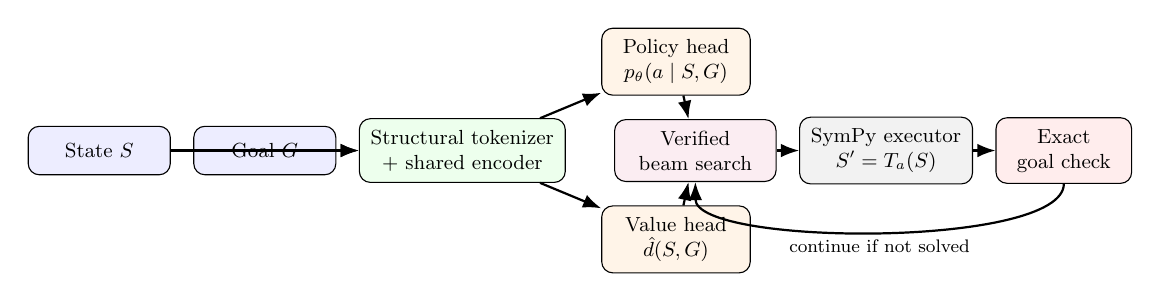
\begin{tikzpicture}[node distance=0.55cm and 0.35cm, transform shape, scale=0.82]
  \node[paperbox, fill=blue!7, minimum width=2.2cm] (state) {State $S$};
  \node[paperbox, fill=blue!7, minimum width=2.2cm, right=of state] (goal) {Goal $G$};
  \node[paperbox, fill=green!7, minimum width=2.8cm, right=of goal] (enc) {Structural tokenizer\\+ shared encoder};
  \node[paperbox, fill=orange!9, minimum width=2.3cm, above right=0.35cm and 0.55cm of enc] (policy) {Policy head\\$p_\theta(a\mid S,G)$};
  \node[paperbox, fill=orange!9, minimum width=2.3cm, below right=0.35cm and 0.55cm of enc] (value) {Value head\\$\hat d(S,G)$};
  \node[paperbox, fill=purple!7, minimum width=2.5cm, right=0.75cm of enc] (beam) {Verified\\beam search};
  \node[paperbox, fill=gray!10, minimum width=2.4cm, right=of beam] (sympy) {\sympy{} executor\\$S'=T_a(S)$};
  \node[paperbox, fill=red!7, minimum width=2.1cm, right=of sympy] (check) {Exact\\goal check};

  \draw[paperarrow] (state) -- (enc);
  \draw[paperarrow] (goal) -- (enc);
  \draw[paperarrow] (enc) -- (policy);
  \draw[paperarrow] (enc) -- (value);
  \draw[paperarrow] (policy) -- (beam);
  \draw[paperarrow] (value) -- (beam);
  \draw[paperarrow] (beam) -- (sympy);
  \draw[paperarrow] (sympy) -- (check);
  \draw[paperarrow] (check.south) .. controls +(0,-1.0) and +(0,-1.0) .. node[paperlabel, below] {continue if not solved} (beam.south);
\end{tikzpicture}
\caption{Verified symbolic rewrite search loop. The model scores actions and progress, but every transition is executed symbolically and every success condition is exactly checked.}
\label{fig:system}
\end{figure}

\section{Models}

All models share a structural tokenizer over symbolic expressions and a common encoder backbone. The current state and goal are encoded as
\[
z_S=E(S), \qquad z_G=E(G),
\]
and fused into
\[
h = [z_S ; z_G ; z_S-z_G ; z_S\odot z_G],
\]
where $\odot$ is elementwise multiplication and $[\cdot;\cdot]$ denotes concatenation. A value head predicts the distance-to-goal estimate $\hat d=v(h)$. The policy head differs by model family.

\subsection{MLP baseline}

The \mlp{} policy head maps $h$ directly to action logits with a small dense network. It is the baseline for whether the structured policy heads add value.

\subsection{Static KAN}

The \staticKAN{} head replaces a dense mapping with spline-based edge functions. Abstractly, each output logit is built from sums of one-dimensional nonlinear edge functions over hidden coordinates:
\[
y_j = \sum_i \phi_{ij}(x_i),
\]
where each $\phi_{ij}$ is represented by a learned spline or a mixture over spline templates. The intended benefit is a stronger inductive bias for structured symbolic decision boundaries than a purely dense policy head.

\subsection{HyperKAN}

\hyperkan{} is a goal-conditioned \kan{} in which a hypernetwork modulates the policy head using the goal embedding. Let $H(\cdot)$ denote the hypernetwork. It maps the goal representation to modulation parameters
\[
m = H(z_G).
\]
For an edge function represented as a mixture over $K$ templates,
\[
\phi_{ij}(x_i\mid z_G)
  = \sum_{k=1}^{K} \alpha_{ij,k}(z_G)\,\psi_{ij,k}(x_i),
\]
where the coefficients $\alpha_{ij,k}(z_G)$ are produced by the hypernetwork and $\psi_{ij,k}$ are learned template functions.

In a later factorized site/op variant, flat action logits are decomposed as
\[
\ell(u,o)=\ell_{\mathrm{site}}(u)+\ell_{\mathrm{op}}(o),
\]
with auxiliary site and operator losses added during training. This variant improves seen-family efficiency but does not solve the held-out mixed family.

\begin{figure}[t]
\centering
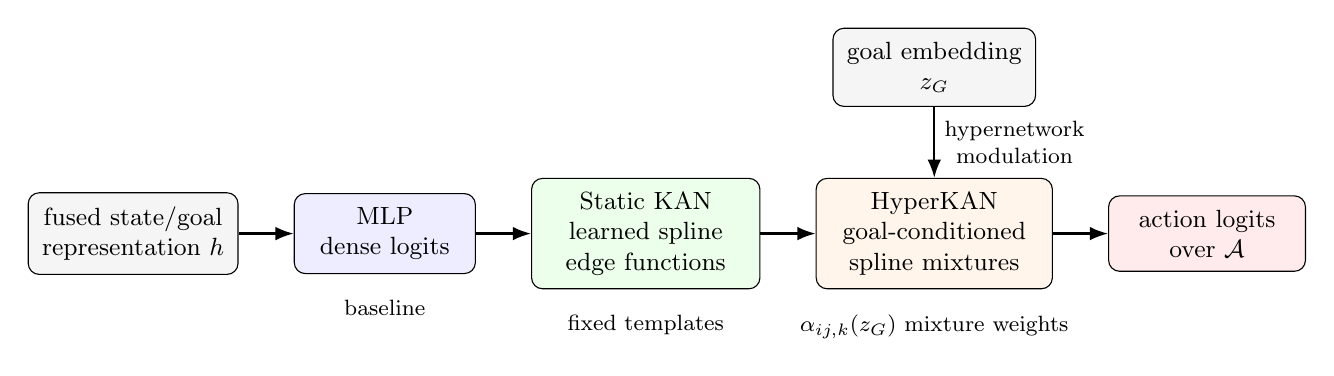
\begin{tikzpicture}[node distance=0.65cm and 0.7cm]
  \node[paperbox, fill=gray!8, minimum width=2.5cm] (h1) {fused state/goal\\representation $h$};
  \node[paperbox, fill=blue!7, minimum width=2.3cm, right=of h1] (mlp) {MLP\\dense logits};
  \node[paperbox, fill=green!8, minimum width=2.9cm, right=of mlp] (static) {Static KAN\\learned spline\\edge functions};
  \node[paperbox, fill=orange!8, minimum width=3.0cm, right=of static] (hyper) {HyperKAN\\goal-conditioned\\spline mixtures};
  \node[paperbox, fill=gray!8, minimum width=2.5cm, above=0.9cm of hyper] (zg) {goal embedding\\$z_G$};
  \node[paperbox, fill=red!8, minimum width=2.5cm, right=of hyper] (logits) {action logits\\over $\mathcal{A}$};

  \draw[paperarrow] (h1) -- (mlp);
  \draw[paperarrow] (mlp) -- (static);
  \draw[paperarrow] (static) -- (hyper);
  \draw[paperarrow] (hyper) -- (logits);
  \draw[paperarrow] (zg) -- node[paperlabel, right] {hypernetwork\\modulation} (hyper);

  \node[paperlabel, below=0.2cm of mlp] {baseline};
  \node[paperlabel, below=0.2cm of static] {fixed templates};
  \node[paperlabel, below=0.2cm of hyper] {$\alpha_{ij,k}(z_G)$ mixture weights};
\end{tikzpicture}
\caption{Policy-head comparison. The models share the same state/goal encoder and value head; the policy head changes from dense logits to static spline edge functions to goal-conditioned spline mixtures.}
\label{fig:policy-heads}
\end{figure}

\section{Training Objective and Inference}

Given action logits $\ell$, let $p_\theta(a\mid S,G)$ denote the model score for action $a$. For multi-label shortest-action supervision we use a binary cross-entropy style action loss over the valid shortest set $A^\star(S,G)$:
\[
\mathcal{L}_{\mathrm{act}}
 = \sum_{a\in\mathcal{A}} \bce\!\left(p_\theta(a\mid S,G),y_a\right),
\quad
y_a=\mathbf{1}[a\in A^\star(S,G)].
\]
For guided single-path scoped datasets, the target is a one-hot action $a^\star(S,G)$.

Distance-to-goal is trained with a Huber regression loss:
\[
\mathcal{L}_{\mathrm{val}}=\huber(\hat d,d(S,G)).
\]
The total loss is
\[
\mathcal{L}
 = \mathcal{L}_{\mathrm{act}}
 + \lambda_{\mathrm{val}}\mathcal{L}_{\mathrm{val}}
 + \mathcal{L}_{\mathrm{aux}},
\]
where $\mathcal{L}_{\mathrm{aux}}$ is zero for the base models and contains optional auxiliary terms in ablation branches, such as site/op supervision or root-avoidance penalties.

\subsection{Beam-search inference}

At inference time, the model is embedded inside beam search. For a partial path $\pi_t=(a_1,\ldots,a_t)$ producing states $S_0,\ldots,S_t$, the shaped search score is
\[
\mathrm{score}(\pi_t)
 =
\sum_{\tau=1}^{t}
\left[
\log p_\theta(a_\tau\mid S_{\tau-1},G)
+ \beta_v\, \hat v(S_\tau,G)
+ b_{\mathrm{root}}(a_\tau,S_{\tau-1})
+ b_{\mathrm{frontier}}(S_\tau,\tau)
\right].
\]
Here $b_{\mathrm{root}}$ is an optional penalty on root-level whole-expression actions and $b_{\mathrm{frontier}}$ is an optional early-frontier bonus used in the reranker experiments. Each proposed action is executed symbolically. Invalid rewrites are discarded. A candidate succeeds only if the executed symbolic state matches the target under the benchmark verification semantics.

\begin{figure}[t]
\centering
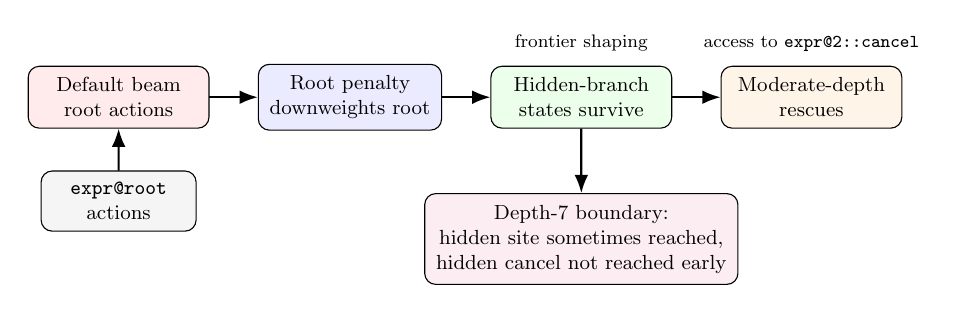
\begin{tikzpicture}[node distance=0.55cm and 0.75cm, transform shape, scale=0.82]
  \node[paperbox, fill=red!8, minimum width=2.8cm] (default) {Default beam\\root actions};
  \node[paperbox, fill=gray!8, minimum width=2.4cm, below=0.65cm of default] (root) {\texttt{expr@root}\\actions};
  \node[paperbox, fill=blue!8, minimum width=2.8cm, right=of default] (penalty) {Root penalty\\downweights root};
  \node[paperbox, fill=green!8, minimum width=2.8cm, right=of penalty] (hidden) {Hidden-branch\\states survive};
  \node[paperbox, fill=orange!9, minimum width=2.8cm, right=of hidden] (solve) {Moderate-depth\\rescues};
  \node[paperbox, fill=purple!7, minimum width=4.4cm, below=1.0cm of hidden] (limit) {Depth-7 boundary:\\hidden site sometimes reached,\\hidden cancel not reached early};

  \draw[paperarrow] (default) -- (penalty);
  \draw[paperarrow] (penalty) -- (hidden);
  \draw[paperarrow] (hidden) -- (solve);
  \draw[paperarrow] (root) -- (default);
  \draw[paperarrow] (hidden) -- (limit);
  \node[paperlabel, above=0.1cm of hidden] {frontier shaping};
  \node[paperlabel, above=0.1cm of solve] {access to \texttt{expr@2::cancel}};
\end{tikzpicture}
\caption{Root-collapse and frontier-shaping mechanism. The root penalty reveals useful local signal in recovered HyperKAN, while the frontier reranker improves the moderate-depth mixed-family result. The depth-7 expansion shows where this mechanism stops converting early frontier changes into solves.}
\label{fig:frontier-mechanism}
\end{figure}

\section{Global Benchmark}

The original verified benchmark contains 274 non-terminal test problems. Beam search uses width 4 and a maximum of 8 steps. Table~\ref{tab:global} reports the main global-action result.

\begin{table}[t]
\centering
\caption{Global-action benchmark results. Depth-2 is saturated for all models; depth-3 is the only real discriminator.}
\label{tab:global}
\begin{tabular}{lrrr}
\toprule
Model & Beam solves & Solve rate & Depth-3 solves \\
\midrule
\mlp{} & 147/274 & 53.6\% & 0/127 \\
\staticKAN{} & 163/274 & 59.5\% & 16/127 \\
\hyperkan{} (initial) & 148/274 & 54.0\% & 1/127 \\
\hyperkan{} (recovered) & 162/274 & 59.1\% & 15/127 \\
\bottomrule
\end{tabular}
\end{table}

\begin{figure}[t]
\centering
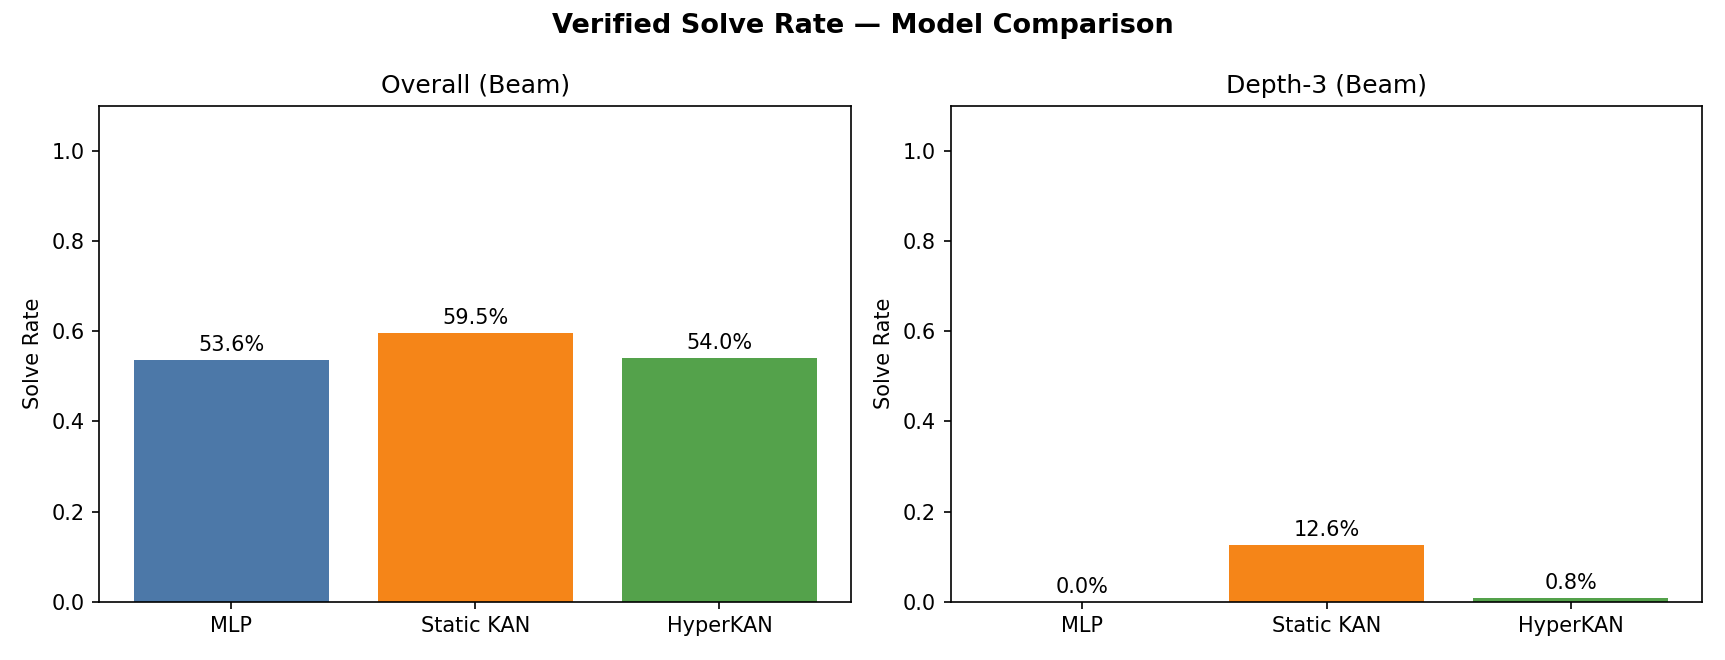
\includegraphics[width=\linewidth]{figures/model_comparison.png}
\caption{Historical global-action benchmark plot. \staticKAN{} is strongest overall, while the initial \hyperkan{} underperforms on depth-3 examples.}
\label{fig:model-comparison}
\end{figure}

\begin{figure}[t]
\centering
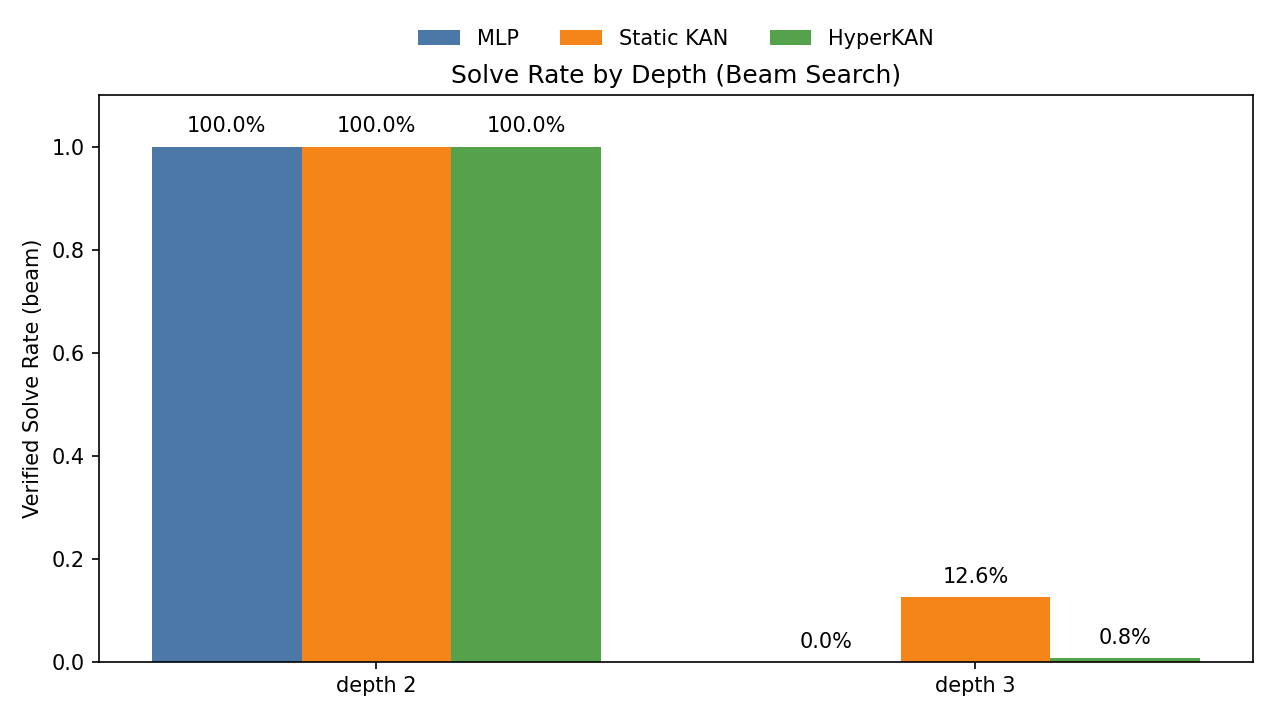
\includegraphics[width=0.82\linewidth]{figures/solve_rate_by_depth.png}
\caption{Depth breakdown for the original global benchmark. Depth-2 is saturated; depth-3 is the only separator. This motivates the later scoped-action redesign.}
\label{fig:depth-global}
\end{figure}

A reduced-capacity \hyperkan{} (\texttt{hyper\_hidden\_dim = 64}) narrows the gap to \staticKAN{}. However, search-temperature calibration does not close the remaining gap, and longer training does not reliably help: verified search can regress even when supervised validation loss continues improving. Thus the global benchmark supports two strong conclusions: \staticKAN{} is better than \mlp{} on the shallow verified benchmark, and supervised validation loss is not a reliable proxy for verified search performance. It does not support broad claims about compositional reasoning because the benchmark is too shallow.

\section{Why Global Actions Fail as a Compositional Benchmark}

We replaced heuristic dataset generation with exact graph mining over typed symbolic families. The graph analysis shows that \texttt{block\_a\_trig\_merge\_expand} yields a verified depth-3 ladder and \texttt{block\_b\_cancel\_expand} yields a verified depth-2 ladder. However, naive additive composition under global whole-expression rewrites does not produce robust depth-4+ families at useful density.

The failure is structural. Global rewrites often simplify multiple latent subproblems at once, collapsing what should be additive depth. This motivates the shift to scoped actions.

\section{Scoped Benchmark Development}

The first scoped datasets were guided plumbing checks. A smoke dataset uses 24 guided trajectories from a depth-4 family and both \staticKAN{} and \hyperkan{} solve 16/16 non-terminal test examples. A medium version scales the same family to 200 trajectories and both models solve 48/48 examples. A diverse guided split adds four action-order families and 400 guided trajectories, but both models still solve 400/400 examples under greedy and beam search.

These results validate the scoped data path, model heads, training loop, checkpointing, and scoped beam evaluation. They also show that guided action-order variation is too templated to test compositional generalization by solve rate.

\section{Structural Scoped Probe}

The first non-saturated scoped benchmark replaces action-order variation with structurally different algebraic families:
\begin{itemize}
  \item \texttt{trig\_merge}: \texttt{trigsimp} $\to$ \texttt{together} $\to$ \texttt{expand},
  \item \texttt{hidden\_cancel}: numerator \texttt{factor} $\to$ \texttt{cancel} $\to$ \texttt{expand},
  \item \texttt{apart\_normalize}: denominator \texttt{factor} $\to$ \texttt{apart},
  \item \texttt{mixed\_trig\_hidden}: composition of a trig block and a hidden-factor block.
\end{itemize}

Train/validation use the first three families. Test consists only of \texttt{mixed\_trig\_hidden}. After search-based checkpoint selection, both \staticKAN{} and recovered \hyperkan{} score 0/60 on the held-out mixed family by default, while seen-family performance remains strong. This benchmark is non-saturated and exposes a real held-out composition gap.

\subsection{Failure mode: root-collapse}

Targeted failure analysis reveals root-action collapse. \staticKAN{} assigns top-1 first action \texttt{expr@root::together} on every mixed-family test row. \hyperkan{} assigns top-1 first action \texttt{expr@root::expand} on every mixed-family test row. Default greedy rollouts remain global and never switch into local blockwise behavior. This shows that the problem is not simply insufficient beam width; the learned policies fail to localize onto independent subproblems inside a composed expression.

\section{Inference-Time Rescue and Mechanism Analysis}

A simple inference-time penalty on root actions has very different effects on the two models. \staticKAN{} remains at 0/60 under root penalty 2.0. Recovered \hyperkan{} rises to 24/60 greedy and 36/60 beam. This establishes that recovered \hyperkan{} contains useful compositional signal that default inference does not surface.

The rescue is not explained by first-step localization alone. Under root penalty 2.0, the top-1 action changes on all 60 mixed-family rows, but solved and unsolved beam rows still share the same penalized top-1 action: \texttt{expr@0::trigsimp}. What separates solved from unsolved rows is the early frontier:
\[
\begin{array}{lrr}
\toprule
\text{Path diagnostic} & \text{Solved rows} & \text{Unsolved rows}\\
\midrule
\text{Reach any hidden site within first 3 actions} & 36/36 & 12/24\\
\text{Reach \texttt{expr@2::cancel} within first 3 actions} & 36/36 & 12/24\\
\bottomrule
\end{array}
\]
Thus the rescue comes from early hidden-branch access, not merely from choosing a better first local site.

Straightforward training-time fixes do not internalize this behavior. A small \texttt{expr@root} avoidance loss does not improve default compositional generalization and weakens the stronger inference-only rescue. A factorized site/op \hyperkan{} head improves seen-family efficiency but still yields 0/60 on the held-out mixed family and preserves the same root-action bias.

\section{Early-Frontier Reranker}

The strongest positive result comes from making the mechanism explicit. We add a frontier-aware inference adjustment that rewards early access to the hidden branch while keeping the root penalty. Table~\ref{tab:structural-rescue} summarizes the moderate-depth structural-probe result.

\begin{table}[t]
\centering
\caption{Held-out \texttt{mixed\_trig\_hidden} structural-probe results. The frontier reranker is the best moderate-depth result but remains an inference-side intervention.}
\label{tab:structural-rescue}
\begin{tabular}{lrrr}
\toprule
Condition & Validation beam-4 & Greedy & Beam-4 \\
\midrule
Default recovered \hyperkan{} & 16/16 & 0/60 & 0/60 \\
Root penalty 2.0 & 16/16 & 24/60 & 36/60 \\
Root penalty 2.0 + frontier reranker & 14/16 & 36/60 & 48/60 \\
\bottomrule
\end{tabular}
\end{table}

An earlier hidden-action bonus improved efficiency without improving solve count and hurt seen-family validation. The later frontier-state reranker improves solve count at moderate depth, but this still should not be read as a fully internalized learned solution. It is an inference-side intervention that makes the hidden branch reachable earlier in search.

\section{Depth-7 Expansion: A Clear Failure Boundary}

To test whether the moderate-depth rescue scales, we add a deeper held-out family, \emph{mixed-trig-hidden-apart}, built from three structural blocks with a guided chain of length 7:
\[
\begin{aligned}
&\texttt{expr@1::trigsimp}\\
&\to \texttt{add\_slice@root[1:3]::together}\\
&\to \texttt{expr@2::expand}\\
&\to \texttt{numerator@3::factor}\\
&\to \texttt{expr@3::cancel}\\
&\to \texttt{denominator@1::factor}\\
&\to \texttt{expr@1::apart}.
\end{aligned}
\]
The depth-expansion probe contains 48 trajectories, 228 rows, 84 non-terminal held-out test attempts, and 14 scoped actions.

\begin{table}[t]
\centering
\caption{Depth-7 held-out expansion results. The frontier reranker no longer improves solve rate over the root-penalty baseline.}
\label{tab:depth7}
\begin{tabular}{lrrr}
\toprule
Condition & Greedy & Beam-4 & Mean beam expansions\\
\midrule
Default & 0/84 & 0/84 & 171.23\\
Root penalty 2.0 & 0/84 & 18/84 & 144.67\\
Root penalty 2.0 + frontier reranker & 0/84 & 18/84 & 150.18\\
\bottomrule
\end{tabular}
\end{table}

All 18 solved beam cases under the successful conditions are the same one-action path, \texttt{expr@1::\allowbreak apart}. Table~\ref{tab:distance-slice} gives the distance-slice failure analysis.

\begin{table}[t]
\centering
\caption{Distance-slice analysis for the depth-7 held-out family. The partial rescue does not traverse the deeper chain.}
\label{tab:distance-slice}
\begin{tabular}{lrrrrrrr}
\toprule
Condition & $d=1$ & $d=2$ & $d=3$ & $d=4$ & $d=5$ & $d=6$ & $d=7$\\
\midrule
Root penalty 2.0 & 9/12 & 0/12 & 9/12 & 0/12 & 0/12 & 0/12 & 0/12\\
Root penalty 2.0 + frontier reranker & 9/12 & 0/12 & 9/12 & 0/12 & 0/12 & 0/12 & 0/12\\
\bottomrule
\end{tabular}
\end{table}

The reranker reaches a hidden site early on 10/84 rows, but reaches hidden cancel within the first 3 actions on 0/84 rows. It reshapes part of the frontier without converting that into deeper hidden-branch solves. This depth-7 probe is therefore a genuine failure boundary. The moderate-depth rescue is real, but it does not carry over cleanly to deeper compositions.

\begin{figure}[t]
\centering
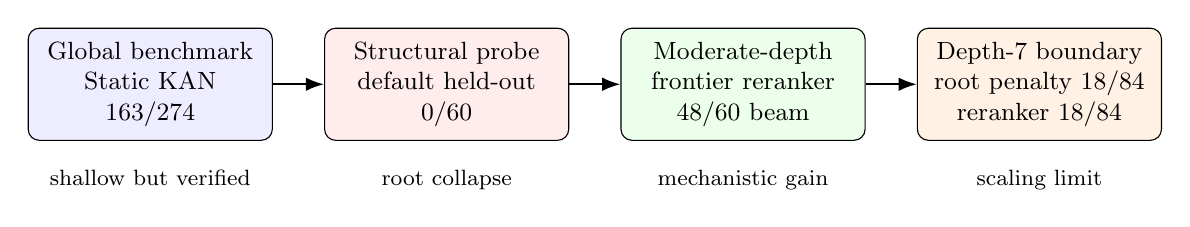
\begin{tikzpicture}[node distance=0.55cm and 0.65cm]
  \node[paperbox, fill=blue!7, minimum width=3.1cm, minimum height=1.35cm] (global) {Global benchmark\\Static KAN\\163/274};
  \node[paperbox, fill=red!7, minimum width=3.1cm, minimum height=1.35cm, right=of global] (gap) {Structural probe\\default held-out\\0/60};
  \node[paperbox, fill=green!8, minimum width=3.1cm, minimum height=1.35cm, right=of gap] (rescue) {Moderate-depth\\frontier reranker\\48/60 beam};
  \node[paperbox, fill=orange!10, minimum width=3.1cm, minimum height=1.35cm, right=of rescue] (depth) {Depth-7 boundary\\root penalty 18/84\\reranker 18/84};
  \draw[paperarrow] (global) -- (gap);
  \draw[paperarrow] (gap) -- (rescue);
  \draw[paperarrow] (rescue) -- (depth);
  \node[paperlabel, below=0.25cm of global] {shallow but verified};
  \node[paperlabel, below=0.25cm of gap] {root collapse};
  \node[paperlabel, below=0.25cm of rescue] {mechanistic gain};
  \node[paperlabel, below=0.25cm of depth] {scaling limit};
\end{tikzpicture}
\caption{Main empirical arc. Global actions provide a verified but shallow starting point; scoped structural probes expose a held-out mixed-family gap; frontier shaping rescues moderate-depth performance; the depth-7 expansion marks the current failure boundary.}
\label{fig:main-summary}
\end{figure}

\section{Concrete Depth-7 Trajectory}

The following held-out trajectory illustrates the depth-expansion setup:
\[
\begin{aligned}
S_0={}&
\frac{5z+16}{z^2+7z+10}
+\left(\frac{4}{x+4}+\frac{3}{x+3}\right)(\sin^2 y+\cos^2 y)\\
&+\frac{z^2+9z+14}{(z+1)(z+2)^2},
\end{aligned}
\]
with target
\[
\begin{aligned}
G={}&
\frac{7x}{x^2+7x+12}
+\left(\frac{3}{z+5}+\frac{2}{z+2}\right)
+\frac{24}{x^2+7x+12}\\
&+\frac{z+7}{(z+1)(z+2)}.
\end{aligned}
\]
The guided action chain has length 7, as listed in the previous section. Under root-penalized beam search, however, the solved depth-expansion rows are the one-action \texttt{expr@1::apart} shortcut cases. The model does not traverse the full seven-action chain, and the frontier reranker does not fix that.

\section{What Is Proven and What Is Not}

\subsection{Supported conclusions}

\begin{itemize}
  \item The original global benchmark works end to end.
  \item \staticKAN{} beats \mlp{} on the global benchmark.
  \item Recovered \hyperkan{} can nearly match \staticKAN{} on the global benchmark.
  \item Verified search metrics can diverge from supervised validation loss.
  \item Scoped action infrastructure works end to end.
  \item The structural scoped probe is non-saturated and exposes a real held-out composition gap.
  \item Root-penalized localization-aware inference is a meaningful official evaluation condition.
  \item Early hidden-branch access within the first 3 actions is a real discriminator on the moderate-depth mixed family.
  \item A frontier-aware reranker improves held-out mixed-family performance from 36/60 beam to 48/60 beam.
  \item The depth-7 expansion exposes a clear failure boundary: root penalty retains a shallow partial rescue, but the frontier reranker no longer improves solve rate.
\end{itemize}

\subsection{Not yet shown}

\begin{itemize}
  \item Robust strict depth-4+ density under scoped exact verification.
  \item Shortest-action multi-label tie recovery for composed scoped cases.
  \item Clean separation between \staticKAN{} and \hyperkan{} under a fully strict scoped benchmark.
  \item A training-time localization objective that internalizes the successful inference-side rescue.
  \item A learned reranker or search-aligned training method that transfers the moderate-depth mechanism to depth-7 traversal.
\end{itemize}

\section{Limitations}

This work has several important limitations. First, the strongest scoped results still rely on guided single-path labels or guided accepted families rather than fully strict composed shortest-action recovery at dataset scale. Second, the successful rescues are inference-side interventions. They provide mechanism insight, but they are not yet clean end-to-end learned solutions. Third, the benchmark remains highly structured. Although the structural probe is stronger than the guided smoke and medium datasets, it is still a controlled symbolic setting rather than a broad theorem-proving benchmark. Fourth, the depth-7 expansion shows that the current rescue mechanism has a limited regime of validity.

\section{Discussion and Positioning}

This paper is best read as a benchmark-and-mechanism paper, not as a claim that \hyperkan{} universally dominates \mlp{} or \staticKAN{}. The strongest positive result is conditional and specific: under a scoped structural probe with real held-out compositional pressure, inference-side frontier shaping materially improves recovered \hyperkan{} on a moderate-depth mixed family. The strongest negative result is equally important: that rescue does not scale cleanly to the deeper depth-7 family, and several obvious training-time localization fixes fail to internalize it.

The contribution is therefore twofold: first, a verified symbolic search benchmark analysis showing why whole-expression action semantics can make composition artificially shallow; second, a mechanistic study of how search-time frontier shaping can partially rescue compositional generalization before a clear failure boundary appears.

\section{Reviewer Questions and Responses}

\paragraph{Is the benchmark too synthetic or templated to say much about reasoning?}
The benchmark is intentionally controlled and synthetic. Its purpose is not to represent all symbolic reasoning, but to isolate how action granularity, search, and model inductive bias interact under exact symbolic verification. The controlled setup is what makes the root-collapse failure mode and the early-frontier rescue measurable.

\paragraph{Why use scoped actions instead of the original global \sympy{} actions?}
Graph analysis shows that whole-expression actions collapse composition. Under global actions, isolated depth-2 and depth-3 ladders exist, but naive composition does not yield robust depth-4+ families at useful density. Scoped actions are therefore the benchmark change required to make compositional structure visible.

\paragraph{Is the inference rescue just a hand-engineered heuristic?}
Yes. The root penalty and frontier reranker are inference-side interventions, not clean end-to-end learned solutions. Their value is diagnostic: they show that recovered \hyperkan{} contains useful signal that default search does not surface, and that early hidden-branch access is a key mechanism.

\paragraph{Why did the training-time localization fixes fail if the inference bias worked?}
The negative result suggests the bottleneck is not generic locality alone. Simple root-avoidance and factorized site/op supervision do not reliably teach the policy to sequence hidden subgoals under held-out composition. The successful inference bias changes the search frontier; the training fixes tested here do not internalize that behavior.

\paragraph{Could a different checkpoint change the conclusion?}
Checkpoint choice matters, which is why the later scoped results use search-based checkpoint selection rather than supervised validation loss alone. The depth-7 result is not a single loss-selected checkpoint artifact: all three depth-expansion inference conditions selected the same checkpoint, isolating the inference behavior.

\paragraph{Do the results prove \hyperkan{} is better than \staticKAN{} or \mlp{}?}
No. On the shallow global benchmark, \staticKAN{} is strongest. Recovered \hyperkan{} becomes competitive but does not clearly dominate. The scoped result is narrower: recovered \hyperkan{} can be substantially rescued by inference-side frontier shaping on a moderate-depth held-out mixed family, while \staticKAN{} does not respond the same way to the simple root penalty tested here.

\paragraph{Why should readers trust a result that depends on beam search and reranking?}
Beam search is the inference procedure under study, not an afterthought. The paper studies learned heuristics for verified symbolic search, so the interaction between model scores and frontier management is part of the phenomenon. The reranker result is reported as an inference-side mechanism result, not as a pure one-step classification result.

\paragraph{Is the depth-7 expansion a failure of the reranker or a failure of the benchmark?}
It is best interpreted as a boundary condition. The moderate-depth rescue is real, but it does not carry over to the deeper family. That strengthens the empirical story: the mechanism helps in one regime and has a measured failure point.

\paragraph{Why not just use brute-force search for these short depths?}
For the shallow settings, brute-force search is plausible. The point of the work is not to replace brute force on depth-3 tasks. It is to study how learned heuristics and action semantics change effective search behavior as compositional pressure increases.

\paragraph{What is the honest takeaway?}
The honest takeaway is that benchmark semantics, action granularity, and frontier shaping materially change what these models appear able to do in verified symbolic rewrite search. Moderate compositional gains can be obtained and analyzed mechanistically, but the current approach has a clear depth boundary and should not be described as solving symbolic reasoning.

\section{Conclusion}

The main lesson of this project is that symbolic benchmark semantics and action granularity matter as much as model class. Whole-expression rewrite actions create shallow composition even when local ladders exist, while scoped actions expose real compositional failure modes. On this scoped benchmark, default policies collapse to root-level actions on held-out mixed compositions. A localization-aware inference bias rescues recovered \hyperkan{}, and a frontier-aware reranker improves held-out moderate-depth compositional performance further, showing that early hidden-branch access is a key mechanism. However, this rescue fails to scale cleanly to a deeper depth-7 family, marking a clear current limit of the approach.

The result is therefore not a claim that \hyperkan{} is universally superior, nor that symbolic reasoning has been solved. It is a more precise claim: learned heuristics for verified symbolic rewrite search are highly sensitive to action granularity, search-time frontier shaping, and benchmark depth, and moderate compositional gains can be obtained and analyzed mechanistically before a clear failure boundary emerges.

\begin{thebibliography}{9}

\bibitem{kan}
Z. Liu et al.
\newblock KAN: Kolmogorov-Arnold Networks.
\newblock arXiv preprint, 2024.

\bibitem{sympy}
A. Meurer et al.
\newblock SymPy: symbolic computing in Python.
\newblock \emph{PeerJ Computer Science}, 2017.

\bibitem{neural-guided-search}
S. Loos, G. Irving, C. Szegedy, and C. Kaliszyk.
\newblock Deep Network Guided Proof Search.
\newblock \emph{LPAR}, 2017.

\bibitem{benchmarking}
F. Chollet.
\newblock On the Measure of Intelligence.
\newblock arXiv preprint, 2019.

\end{thebibliography}

\appendix
\section{Current Best Results Summary}

\begin{center}
\begin{tabular}{>{\raggedright\arraybackslash}p{0.25\linewidth}>{\raggedright\arraybackslash}p{0.43\linewidth}>{\raggedright\arraybackslash}p{0.22\linewidth}}
\toprule
Setting & Best condition & Outcome\\
\midrule
Global benchmark & \staticKAN{} & 163/274 (59.5\%)\\
Moderate-depth mixed-family scoped benchmark & \hyperkan{} + root penalty 2.0 + frontier reranker & 48/60 beam, 36/60 greedy\\
Moderate-depth mechanism & Early hidden-branch access & solved rows: 36/36 reach hidden cancel within 3 actions\\
Depth-7 scoped expansion & \hyperkan{} + root penalty 2.0 & 18/84 beam\\
\bottomrule
\end{tabular}
\end{center}

\section{Reproduction Notes}

All ROCm training and evaluation commands run inside the \texttt{llama-rocm-7.2} toolbox environment. The repository contains scripts and configs for global benchmark generation and evaluation, scoped smoke/medium/diverse datasets, the scoped structural probe, search-based checkpoint selection, mixed-family failure analysis, early-frontier mechanism analysis, and the depth-expansion probe. The branch README records the current command set and artifact layout.

\end{document}
